%%%%%%%%%%%%%%%%%%%%%%%%%%%%%%%%%%%%%%%%%%%%%%%%%%%%%%%%%%%%%%%%%%%%%%
% CS637: Database-Backed Websites
% Copyright 2015 Pejman Ghorbanzade <mail@ghorbanzade.com>
% Creative Commons Attribution-ShareAlike 4.0 International License
% More info: https://bitbucket.org/ghorbanzade/umb-cs637-2015s
%%%%%%%%%%%%%%%%%%%%%%%%%%%%%%%%%%%%%%%%%%%%%%%%%%%%%%%%%%%%%%%%%%%%%%

\section*{Question 4}

\begin{enumerate}[label=(\alph*)]
\item Consider the \texttt{index.html} available at \href{http://topcat.cs.umb.edu/book\_apps/ch01\_product\_discount}{here}, where it is displayed using the book's \texttt{main.css}. A different \texttt{main.css} is used to display it as shown in \ref{fig2}. Note the following: different colors, different font styles, different font sizes, wider overall (600px), more space around contents, wider border. Write a CSS file that shows at least approximately this display and show it in your paper.

\begin{figure}\centering
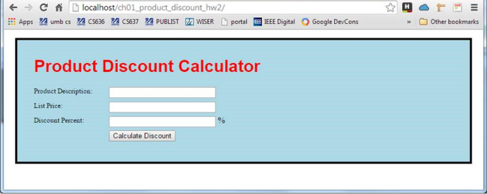
\includegraphics{\pngDirectory/hw02/hw02q04f02.png}
\caption{Front-End of Product Discount Calculator as Given}\label{fig2}
\end{figure}

\item If you have a Windows system, describe how the above-mentioned \href{http://topcat.cs.umb.edu/book_apps/ch01_product_discount/}{page} shows in your version of Internet Explorer.
\end{enumerate}

\subsection*{Solution}

\begin{enumerate}[label=(\alph*)]
\item The web-page has been redesigned to appear just as identical as possible to the front-end given in Figure \ref{fig2}. The redesigned form is shown in \ref{fig3}.

\begin{figure}\centering
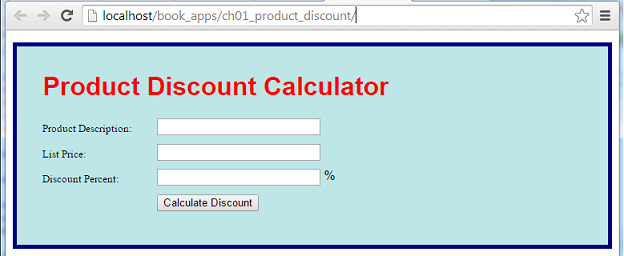
\includegraphics{\pngDirectory/hw02/hw02q04f03.png}
\caption{Redesigned version of Product Discount Calculator}
\label{fig3}
\end{figure}

And the \textit{CSS} code to convert the front-end given by the book application to what it is now is shown below.

\begin{lstlisting}
%\begin{minted}[fontsize=\small,tabsize=8,linenos, firstnumber=1,frame=lines,framerule=1pt]{css}
body {
    font-family: Arial, Helvetica, sans-serif;
}
main {
    width: 90%;
    margin: 15px auto;
    padding: 2em;
    background: rgb(190, 230, 231);
    border: 5px solid navy;
}
h1 {
    margin-top: 0;
    color: red;
}
label {
    width: 10em;
    float: left;
    padding-right: 1em;
    padding-bottom: .5em;
    line-height: 25px;
    font-family: initial;
    font-size: 13px;
}
#data input {
    float: left;
    width: 15em;
    margin-bottom: .5em;
}
#data span {
    padding-left: .25em;
}
#buttons input {
    float: left;
    margin-bottom: .5em;
}
br {
    clear: left;
}
%\end{minted}
\end{lstlisting}

\item Although all browsers load the same source page, they interpret CSS differently and thus give possibly different presentations of a certain page. Internet Explorer, for instance, presented the web page with following differences. The web page looks as depicted in Figure \ref{fig4} in Internet Explorer.

\begin{enumerate}[label=\arabic*.]
\item The \texttt{margin: auto;} property is not recognized and thus the form is not aligned at the center.
\item The border property of the \texttt{<main>} element has been disregarded.
\item hovering over input elements of the form would change default border color of the elements to light blue.
\item hovering over \texttt{input[type=submit]} element changes its background color to light blue.
\item focusing on \texttt{input[type=text]} elements does not change their \texttt{outline}.
\end{enumerate}

\begin{figure}[H]\centering
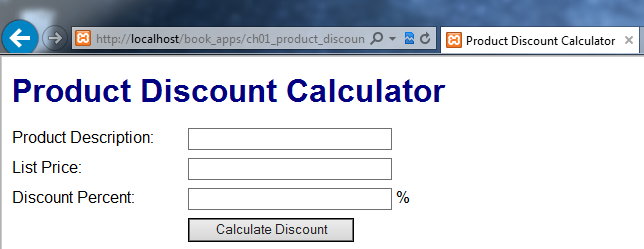
\includegraphics{\pngDirectory/hw02/hw02q04f04.png}
\caption{Front-end view of Product Discount Calculator using Internet Explorer v10.0.9200.16635}\label{fig4}
\end{figure}

\end{enumerate}
